% !Mode:: "TeX:UTF-8"
% 七年级上学期第一单元三视图

\begin{defproblem}{7NJ-01-01}%
\begin{onlyproblem}%
在利用三视图确定小木块个数时,数字一般标在\underline{\hspace*{2cm}}图上.

\end{onlyproblem}%
\begin{onlysolution}%
\begin{solution}%%
俯视
\end{solution}%
\end{onlysolution}%
\end{defproblem}





\begin{defproblem}{7NJ-01-02}%
\begin{onlyproblem}%
观察一个几何体的形状通常从三个方向看,从正面看(主视图),从左面看(左视图),从上面看(俯视图),

从正面看可以看到几何体的\underline{\hspace*{2cm}}和\underline{\hspace*{2cm}};

从左面看可以看到几何体的\underline{\hspace*{2cm}}和\underline{\hspace*{2cm}};

从上面看可以看到几何体的\underline{\hspace*{2cm}}和\underline{\hspace*{2cm}}.
\end{onlyproblem}%
\begin{onlysolution}%
\begin{solution}%%
从正面看可以看到几何体的列数和层数;
从左面看可以看到几何体的行数和层数;
从上面看可以看到几何体的列数和行数.
\end{solution}%
\end{onlysolution}%
\end{defproblem}




\begin{defproblem}{7NJ-01-03}%
\begin{onlyproblem}%
如图是一个由多个相同小立方块堆积而成的几何体的俯视图,图中所示数字为该位置小立方块的个数,则这个几何体的主视图是(    )
\begin{center}
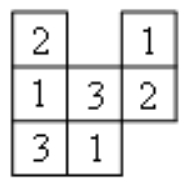
\includegraphics[width=2cm]{7NJ01-01-20190802-1.jpg}
\end{center}

\begin{center}
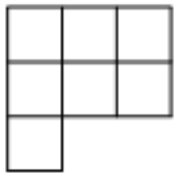
\includegraphics[width=2cm]{7NJ01-01-20190802-2.jpg}
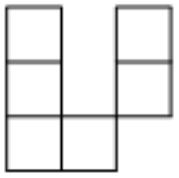
\includegraphics[width=2cm]{7NJ01-01-20190802-3.jpg}
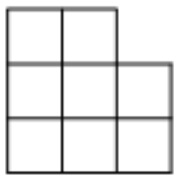
\includegraphics[width=2cm]{7NJ01-01-20190802-4.jpg}
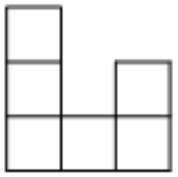
\includegraphics[width=2cm]{7NJ01-01-20190802-5.jpg}
\end{center}

\end{onlyproblem}%
\begin{onlysolution}%
\begin{solution}%%
C
\end{solution}%
\end{onlysolution}%
\end{defproblem}




\begin{defproblem}{7NJ-01-04}%
\begin{onlyproblem}%
如图所示是由一些相同的小正方体构成的几何体的三视图,则这些相同的小正方体的个数是(    )
\begin{center}
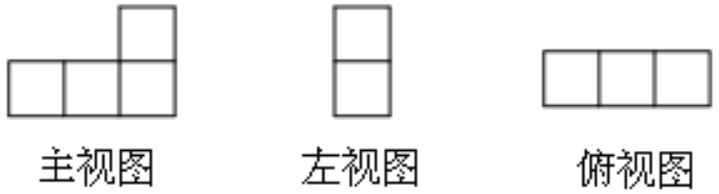
\includegraphics[width=5cm]{7NJ01-01-20190802-6.jpg}
\end{center}

\xx
{3个}
{4个}
{5个}
{6个}

\end{onlyproblem}%
\begin{onlysolution}%
\begin{solution}%%
B
\end{solution}%
\end{onlysolution}%
\end{defproblem}



\begin{defproblem}{7NJ-01-05}%
\begin{onlyproblem}%
如图所示是由一些相同的小正方体构成的几何体的三视图,这些相同的小正方体的个数是(    )
\begin{center}
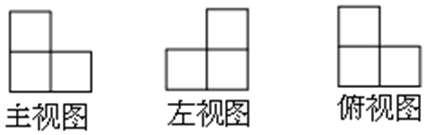
\includegraphics[width=5cm]{7NJ01-01-20190802-7.jpg}
\end{center}

\xx
{3个}
{4个}
{5个}
{6个}

\end{onlyproblem}%
\begin{onlysolution}%
\begin{solution}%%
B
\end{solution}%
\end{onlysolution}%
\end{defproblem}




\begin{defproblem}{7NJ-01-06}%
\begin{onlyproblem}%
用小正方体搭建成的几何体,下面三个图分别是它的主视图、左视图和俯视图,那么构成这个几何体的小正方体有(    )
\begin{center}
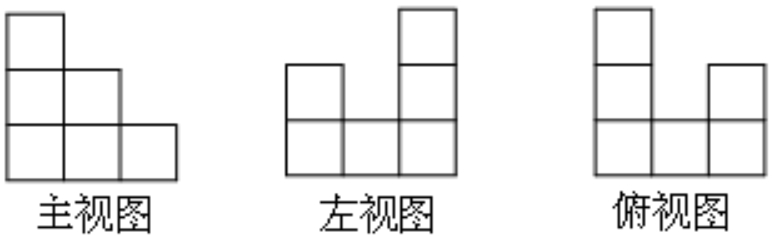
\includegraphics[width=5cm]{7NJ01-01-20190802-8.jpg}
\end{center}

\xx
{6个}
{9个}
{10个}
{11个}

\end{onlyproblem}%
\begin{onlysolution}%
\begin{solution}%%
B
\end{solution}%
\end{onlysolution}%
\end{defproblem}



\begin{defproblem}{7NJ-01-07}%
\begin{onlyproblem}%
由若干个相同的小正方体搭成的一个几何体的主视图和俯视图如图所示,则组成这个几何体的小正方体的个数最少有(    )
\begin{center}
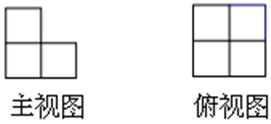
\includegraphics[width=5cm]{7NJ01-01-20190802-9.jpg}
\end{center}

\xx
{4个}
{5个}
{6个}
{7个}


\end{onlyproblem}%
\begin{onlysolution}%
\begin{solution}%%
B
\end{solution}%
\end{onlysolution}%
\end{defproblem}




\begin{defproblem}{7NJ-01-08}%
\begin{onlyproblem}%
如图是由一些大小相同的小正方体搭成的一个几何体的左视图和俯视图,则组成这个几何体的小正方体的个数最多有(    )
\begin{center}
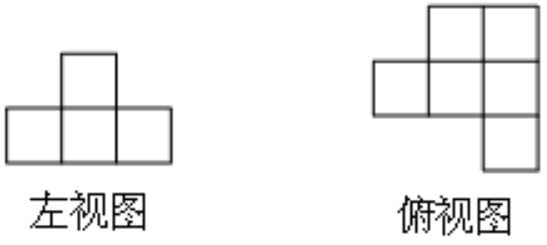
\includegraphics[width=5cm]{7NJ01-01-20190802-10.jpg}
\end{center}

\xx
{5个}
{6个}
{8个}
{9个}


\end{onlyproblem}%
\begin{onlysolution}%
\begin{solution}%%
C
\end{solution}%
\end{onlysolution}%
\end{defproblem}



\begin{defproblem}{7NJ-01-09}%
\begin{onlyproblem}%
用小正方体积木搭出一个主视图和俯视图如图所示的几何体,它最多需要(    )个小正方体积木.
\begin{center}
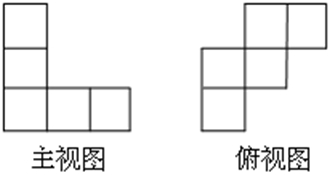
\includegraphics[width=5cm]{7NJ01-01-20190802-11.jpg}
\end{center}

\xx
{8个}
{9个}
{10个}
{11个}


\end{onlyproblem}%
\begin{onlysolution}%
\begin{solution}%%
B
\end{solution}%
\end{onlysolution}%
\end{defproblem}




\begin{defproblem}{7NJ-01-10}%
\begin{onlyproblem}%
一个几何体是由若干个相同的小正方体组成的,其主视图和左视图如图所示,则这个几何体最多可由(    )个这样的小正方体组成. 
\begin{center}
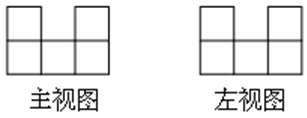
\includegraphics[width=5cm]{7NJ01-01-20190804-01}
\end{center}

\xx
{12}
{13}
{14}
{18}

\end{onlyproblem}%
\begin{onlysolution}%
\begin{solution}%%
B. 
由主视图和左视图确定行数和列数,得到俯视图是几行几列, 然后确定俯视图中每个位置的小正方体的个数,我们选择在俯视图上标数. 根据主视图确定每一列最多有多少层,根据左视图确定每一行最多有多少层, 然后确定每个位置的小正方体的个数. 由主视图和左视图可得该几何体是3行3列, 且第1列最多2层,第2列最多1层,第3列最多2层; 第1行最多2层,第2行最多1层,第3行最多2层,如图所示,
\begin{center}
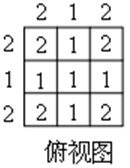
\includegraphics[width=2.5cm]{7NJ01-01-20190804-02}
\end{center}
当小正方体最多时,确定每一个位置上小正方体的个数, 第1行最多2个,第1列最多2个,因此第1行第1列的位置上最多有2个; 第1行最多2个,第2列最多1个,因此第1行第2列的位置上有1个, 依次类推可以得到其他位置上的小正方体的个数.如图所示,   因此小正方体的个数最多有$2\times4+1\times5=13$(个). 
\end{solution}%
\end{onlysolution}%
\end{defproblem}




\begin{defproblem}{7NJ-01-11}%
\begin{onlyproblem}%
如图是由若干个完全相同的小正方体组成的一个几何体的主视图和左视图,则组成这个几何体的小正方体最多有(    ) 
\begin{center}
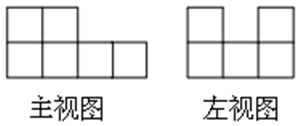
\includegraphics[width=5cm]{7NJ01-01-20190804-30}
\end{center}

\xx
{16个}
{14个}
{19个}
{17个}

\end{onlyproblem}%
\begin{onlysolution}%
\begin{solution}%%
A. 
分析:由主视图和左视图确定行数和列数,得到俯视图是几行几列,然后确定俯视图中每个位置上小正方体的个数,我们选择在俯视图上标数. 从主视图和左视图可得该几何体是3行4列,且第1列最多2层,第2列最多2层,第3列最多1层,第4列最多1层;第1行最多2层,第2行最多1层,第3行最多2层,如下图,
\begin{center}
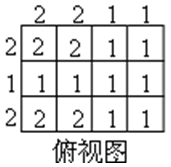
\includegraphics[width=3cm]{7NJ01-01-20190804-31}
\end{center} 
当小正方体最多时,确定每一个位置上小正方体的个数,如下图,   因此,小正方体最多有$2\times4+1\times8=16$(个). 故选A. 
试题难度:三颗星知识点:由三视图求最多、最少问题  

\end{solution}%
\end{onlysolution}%
\end{defproblem}




\begin{defproblem}{7NJ-04-06}%
\begin{onlyproblem}%
将棱长为1的小正方体组成如图所示的几何体,已知该几何体共由8个小正方体组成,则该几何体的表面积是(    )平方单位. 
\begin{center}
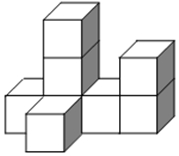
\includegraphics[width=3cm]{7NJ01-04-20190803-09}
\end{center}

\xx
{34}
{32}
{27}
{25}

\end{onlyproblem}%
\begin{onlysolution}%
\begin{solution}%%
A. 根据三视图中小正方体的个数和凹进去的部分, 几何体的表面积为$[(7+4+5) \times 2+2] \times 1^{2}=34$. 故选A. 
\end{solution}%
\end{onlysolution}%
\end{defproblem}




\begin{defproblem}{7NJ-03-05}%
\begin{onlyproblem}%
5个棱长为1的正方体组成如图所示的几何体,则几何体的表面积为(    ) 
\begin{center}
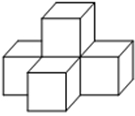
\includegraphics[width=2cm]{7NJ01-03-20190803-06.jpg}
\end{center}

\xx
{18}
{20}
{22}
{16}

\end{onlyproblem}%
\begin{onlysolution}%
\begin{solution}%%
根据三视图中小正方形的个数,几何体的表面积为$(4+3+4) \times 2 \times 1^{2}=22$.
选C.
\end{solution}%
\end{onlysolution}%
\end{defproblem}




\begin{defproblem}{7NJ-03-06}%
\begin{onlyproblem}%
6个棱长为2的小正方体组成如图所示的几何体,则该几何体的表面积为(    ) 
\begin{center}
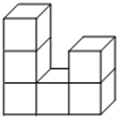
\includegraphics[width=2.3cm]{7NJ01-03-20190803-07.jpg}
\end{center}

\xx
{104}
{26}
{108}
{96}

\end{onlyproblem}%
\begin{onlysolution}%
\begin{solution}%%
选A. 
该几何体的表面积也就是从上、下、左、右、前、后六个方向看到的表面积,再加上凹陷进去的部分. 该几何体的三视图如下,   根据三视图中小正方形的个数和凹陷进去的部分, 几何体的表面积为$[(6+3+3) \times 2+2] \times 2^{2}=104$. 
\end{solution}%
\end{onlysolution}%
\end{defproblem}



\begin{defproblem}{7NJ-03-07}%
\begin{onlyproblem}%
如图是一个由棱长为2cm的正方体组成的几何体的俯视图,小正方形中的数字表示在该位置的正方体的个数,则这个几何体的表面积为(    ) 
\begin{center}
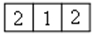
\includegraphics[width=2cm]{7NJ01-03-20190803-08.jpg}
\end{center}
\xx
{68 cm$^2$}
{70 cm$^2$}
{88 cm$^2$}
{90 cm$^2$}

\end{onlyproblem}%
\begin{onlysolution}%
\begin{solution}%%
选C.
利用俯视图,可以画出它的主视图和左视图.   根据三视图中小正方形的个数和凹陷进去的部分, 几何体的表面积为$[(5+2+3) \times 2+2] \times 2^{2}=88 \mathrm{cm}^{2}$. 故选C. 
\end{solution}%
\end{onlysolution}%
\end{defproblem}

